% !TEX root = main.tex
% ------------------------------------------------------------------------
% ------------------------------------------------------------------------
% Modelo UNIAVAN para Trabalhos Acadêmicos baseado em Modelo UFSC de 
% Alisson Lopes Furlani utilizando a classe abntex2
%
% Autor: Luiz Fernando Marquez Arruda
%
% Olá caro autor, leia o arquivo Leia-me.txt
%
%
% Atenciosamente 
%
% Luiz Fernando M. Arruda -  13/06/2024

% ------------------------------------------------------------------------
% ------------------------------------------------------------------------

\documentclass[% -- opções da classe uniavan --
	12pt,				% tamanho da fonte
	openright,			% capítulos começam em pág ímpar (insere página vazia caso preciso)
	oneside,			% para impressão no anverso. Oposto a twoside
	% -- opções da classe abntex2 --
	chapter=TITLE,		% títulos de capítulos convertidos em letras maiúsculas
	section=TITLE,		% títulos de seções convertidos em letras maiúsculas
	%subsection=TITLE,	% títulos de subseções convertidos em letras maiúsculas
	%subsubsection=TITLE,% títulos de subsubseções convertidos em letras maiúsculas
	% -- opções do pacote babel --
	english,			% idioma adicional para hifenização
	%french,			% idioma adicional para hifenização
	%spanish,			% idioma adicional para hifenização
	brazil				% o último idioma é o principal do documento
	]{setup/uniavan}

\addbibresource{references.bib} % Seus arquivos de referências

% -------------------------------------------------------------------------
% Inclusão de novas bibliotecas
% -------------------------------------------------------------------------
% Inclusão de novas bibliotecas devem ser feitas arquivo setup/my_packages.tex
% -----------------------------

% Pacotes personalizados para o projeto
% \usepackage[acronym]{glossaries}

% -------------------------------------------------------------------------
% Dados gerais do documento
% -------------------------------------------------------------------------
% Inclusão do nome do autor, título, orientador, membros da banca, curso etc
% Devem ser editados no arquivo setup/information.tex
% -----------------------------

% ---
% Informações de dados para CAPA e FOLHA DE ROSTO
% ---
% FIXME Substituir 'Nome completo do autor' pelo seu nome.
\autor{MATHEUS GUSTAVO COPPI DA SILVA}
% FIXME Substituir 'Título do trabalho' pelo título da trabalho.
\titulo{Uma arquitetura baseada em microsserviços centrada na
observabilidade}
% FIXME Substituir 'Subtítulo (se houver)' pelo subtítulo da trabalho.  
% Caso não tenha substítulo, comente a linha a seguir.
\subtitulo{}
% FIXME Substituir 'XXXXXX' pelo nome do seu
% orientador.
\orientador{Prof. Luiz Fernando Arruda, Msc}
% FIXME Se for orientado por uma mulher, comente a linha acima e descomente a linha a seguir.
% \orientador[Orientadora]{Nome da orientadora, Dra.}
% FIXME Substituir 'XXXXXX' pelo nome do seu
% coorientador. Caso não tenha coorientador, comente a linha a seguir.
%\coorientador{Prof. XXXXXX, Dr.}
% FIXME Se for coorientado por uma mulher, comente a linha acima e descomente a linha a seguir.
% \coorientador[Coorientadora]{XXXXXX, Dra.}
% FIXME Substituir '[ano]' pelo ano (ano) em que seu trabalho foi defendido.
\ano{2025}
% FIXME Substituir '[dia] de [mês] de [ano]' pela data em que ocorreu sua defesa.
\data{28 de maio de 2025}
% FIXME Substituir 'Local' pela cidade em que ocorreu sua apresentação.
\local{Balneário Camboriú}
% FIXME Substituir 'XXXXXX' pelo nome do coordenador do curso.
\coordenador{Prof. André Moura de Mello, Msc}
% FIXME Se for coordenador por mulher, comente a linha acima e descomente a linha a seguir.
%\coordenador[Coordenadora]{XXXXXX, Dra.}
% FIXME Substituir '[Sigla]' pela sigla da faculdade.
\instituicaosigla{UNIAVAN}
% FIXME Substituir '[Nome da Faculdade]' pelo nome da faculdade.
\instituicao{Centro Universitário Avantis}
% FIXME Substituir '[Tipo de Trabalho]' pelo tipo de trabalho (Trabalho de Conclusão de Curso, Tese, Dissertação). 
\tipotrabalho{Bacharel}
% FIXME Substituir '[Título Escolar]' pela grau adequado (Doutor/Mestre/Especialista/Bacharel/Licenciatura/Tecnólogo em XX).
\formacao{Bacharel em Sistemas de informação}
% FIXME Substituir '[Nível]' pelo nível adequado (Tecnólogo / Graduação / Mestrado / Doutorado).
\nivel{Graduação}
% FIXME Substituir '[Nome do curso]' pelo nome curso adequado.
\curso{Sistemas de informação}

\preambulo
{%
%\imprimirtipotrabalho~apresentado ao curso de~\imprimircurso~do~\imprimirinstituicao~de Balneário Camboriú para a obtenção do título de~\imprimirformacao~em~\imprimircurso.
\imprimirtipotrabalho~apresentado ao curso de~\imprimircurso~do~\imprimirinstituicao~de Balneário Camboriú para a obtenção do título de~\imprimirformacao.
}
% ---

% ---
% Configurações de aparência do PDF final
% ---
% alterando o aspecto da cor azul
\definecolor{blue}{RGB}{41,5,195}
% informações do PDF
\makeatletter
\hypersetup{
     	%pagebackref=true,
		pdftitle={\@title}, 
		pdfauthor={\@author},
    	pdfsubject={\imprimirpreambulo},
	    pdfcreator={LaTeX with abnTeX2},
		pdfkeywords={ufsc, latex, abntex2}, 
		colorlinks=true,       		% false: boxed links; true: colored links
    	linkcolor=black,%blue,          	% color of internal links
    	citecolor=black,%blue,        		% color of links to bibliography
    	filecolor=black,%magenta,      		% color of file links
		urlcolor=black,%blue,
		bookmarksdepth=4
}
\makeatother
% ---

% ---
% carregar e compilar a lista de abreviaturas e siglas e a lista de símbolos
% ---

% carrega a lista de abreviaturas e siglas e a lista de símbolos
% Lista de abreviaturas e siglas
\newacronym{API}{API}{Application Programming Interface}
\newacronym{SOA}{SOA}{Service-Oriented Architecture}
\newacronym{REST}{REST}{Representational State Transfer}
\newacronym{SOAP}{SOAP}{Simple Object Access Protocol}
\newacronym{DevOps}{DevOps}{Development and Operations}
\newacronym{gRPC}{gRPC}{gRPC Remote Procedure Calls}
\newacronym{GraphQL}{GraphQL}{Graph Query Language}
\newacronym{HTTP}{HTTP}{Hypertext Transfer Protocol}
\newacronym{TLS}{TLS}{Transport Layer Security}
\newacronym{DDD}{DDD}{Domain-Driven Design}
\newacronym{UI}{UI}{User Interface}
\newacronym{ML}{ML}{Machine Learning}
\newacronym{EFK}{EFK}{Elasticsearch, Fluentd, Kibana}
\newacronym{ELK}{ELK}{Elasticsearch, Logstash, Kibana}
\newacronym{MVP}{MVP}{Minimum Viable Product}
\newacronym{URI}{URI}{Uniform Resource Identifier}
\newacronym{JSON}{JSON}{JavaScript Object Notation}
\newacronym{XML}{XML}{eXtensible Markup Language}
\newacronym{CPU}{CPU}{Central Processing Unit}
\newacronym{HATEOAS}{HATEOAS}{Hypermedia as the Engine of Application State}
\newacronym{HTTP/2}{HTTP/2}{Hypertext Transfer Protocol version 2}

% Lista de símbolos (opcional)
%\newglossaryentry{symbol:sigma}{name={\sigma}, description={Razão adimensional}}

% compila a lista de abreviaturas e siglas e a lista de símbolos
\makenoidxglossaries 

% ---

% ---
% compila o indice
% ---
\makeindex
% ---

% ----
% Início do documento
% ----
\begin{document}

% Seleciona o idioma do documento (conforme pacotes do babel)
%\selectlanguage{english}
\selectlanguage{brazil}

% Retira espaço extra obsoleto entre as frases.
\frenchspacing 

% Espaçamento 1.5 entre linhas
\OnehalfSpacing

% Corrige justificação
%\sloppy

% -------------------------------------------------------------------------
% ELEMENTOS PRÉ-TEXTUAIS
% -------------------------------------------------------------------------
% Capa, folha de rosto, ficha bibliográfica, errata, folha de aprovação
% Dedicatória, agradecimentos, epígrafe, resumos, listas
% -------------------------------------------------------------------------
% Capa
% -------------------------------------------------------------------------
\imprimircapa
% -------------------------------------------------------------------------


% -------------------------------------------------------------------------
% Folha de rosto
% (o * indica que haverá a ficha bibliográfica)
% -------------------------------------------------------------------------
\imprimirfolhaderosto
% -------------------------------------------------------------------------

% -------------------------------------------------------------------------
% Folha de aprovação
% -------------------------------------------------------------------------
% A folha de aprovação é feita em arquivo separado (para facilitar a impressão / eventual mudança de membro pelo suplente / inclusão da folha escaneada).
% O arquivo de edição da folha de aprovação  está em beforetext/aprovacao.tex
% -------------------------------------------------------------------------
%\begin{folhadeaprovacao}
	\OnehalfSpacing
	\centering
	\imprimirautor\\%
	\vspace*{10pt}		
	\textbf{\imprimirtitulo}%
	\ifnotempty{\imprimirsubtitulo}{:~\imprimirsubtitulo}\\%
	%		\vspace*{31.5pt}%3\baselineskip
	\vspace*{\baselineskip}
	%\begin{minipage}{\textwidth}
	O presente trabalho em nível de~\imprimirnivel~foi avaliado e aprovado por banca examinadora composta pelos seguintes membros:\\
	%\end{minipage}%
	\vspace*{\baselineskip}
	Prof.(a) xxxx, Dr(a).\\
	Instituição xxxx\\
	\vspace*{\baselineskip}
	Prof.(a) xxxx, Dr(a).\\
	Instituição xxxx\\
	\vspace*{\baselineskip}
	Prof.(a) xxxx, Dr(a).\\
	Instituição xxxx\\
	\vspace*{2\baselineskip}
	\begin{minipage}{\textwidth}
		Certificamos~que~esta~é~a~\textbf{versão~original~e~final}~do~\imprimirtipotrabalho~que~foi~julgado~adequado~para~obtenção~do~título~de~\imprimirformacao.\\
	\end{minipage}
	%    \vspace{-0.7cm}
	\vspace*{\fill}
	\assinatura{\OnehalfSpacing~\imprimircoordenador \\ \imprimircoordenadorRotulo~do~Curso de~\imprimirnivel~em~\imprimircurso}
	\vspace*{\fill}
	\assinatura{\OnehalfSpacing\imprimirorientador \\ \imprimirorientadorRotulo}
	%	\ifnotempty{\imprimircoorientador}{
	%	\assinatura{\imprimircoorientador \\ \imprimircoorientadorRotulo \\
	%		\imprimirinstituicao~--~\imprimirinstituicaosigla}
	%	}
	% \newpage
	\vspace*{\fill}
	\imprimirlocal, \imprimirano.
\end{folhadeaprovacao}
%\includepdf{beforetext/aprovacao.pdf}
% -------------------------------------------------------------------------


% -------------------------------------------------------------------------
% Elementos pré-textuais não obrigatórios
% -------------------------------------------------------------------------
% Os elementos pré-textuais devem ser editados na pasta beforetext
% -------------------------------------------------------------------------
% Agradecimentos
% -------------------------------------------------------------------------
%\begin{agradecimentos}

Elemento opcional. Deve aparecer o título centralizado, corpo 12, espacejamento 1,5, negrito e em letras maiúsculas. O texto deve ser justificado com espacejamento de 1,5, fonte 12 e dois espaços 1,5 entre o título.

\end{agradecimentos}
% -------------------------------------------------------------------------


% -------------------------------------------------------------------------
% Epígrafe
% -------------------------------------------------------------------------
%\begin{epigrafe}
	\vspace*{\fill}
    \begin{quoting}[rightmargin=0cm,leftmargin=8cm]
        \noindent A epígrafe é opcional. Apesar de ser escrita por outra pessoa, não deve vir entre aspas. Deve estar localizada na parte inferior direita da folha, utilizando-se fonte 10, espacejamento simples, alinhado a partir do meio da mancha (8 cm) para a margem direita. Referenciar o autor e ano sem parênteses.
		\newline
		\newline
		Nome do autor
    \end{quoting}
\end{epigrafe}
% -------------------------------------------------------------------------

% -------------------------------------------------------------------------
% Resumo
% -------------------------------------------------------------------------
% resumo em português
\setlength{\absparsep}{18pt} % ajusta o espaçamento dos parágrafos do resumo
\begin{resumo}
	\SingleSpacing
	A crescente complexidade dos sistemas e a demanda por escalabilidade impulsionaram a adoção da arquitetura de microsserviços em detrimento do modelo monolítico. Essa abordagem favorece a modularização, a escalabilidade granular e a autonomia das equipes de desenvolvimento, mas também impõe desafios operacionais e de observabilidade. Neste Trabalho de Conclusão de Curso, realiza-se uma comparação entre os protocolos de comunicação \textit{REST} e \textit{gRPC} em arquiteturas baseadas em microsserviços, utilizando métricas de observabilidade como latência (P95 e P99), \textit{throughput} e uso de recursos. A metodologia envolve a implementação de dois serviços equivalentes, instrumentação com Prometheus, execução de testes de carga e análise estatística dos resultados. O objetivo é identificar o protocolo mais eficiente em diferentes cenários de uso. Os resultados esperados visam fornecer subsídios técnicos para orientar decisões arquiteturais em sistemas distribuídos, promovendo um equilíbrio entre desempenho e flexibilidade.
	
	\textbf{Palavras-chave}: microsserviços. \textit{REST}. \textit{gRPC}.
\end{resumo}
% -------------------------------------------------------------------------


% -------------------------------------------------------------------------
% Abstract
% -------------------------------------------------------------------------
\begin{resumo}[Abstract]
	\SingleSpacing
	\begin{otherlanguage*}{english}
		The increasing complexity of systems and the demand for scalability have driven the adoption of microservices architecture over the monolithic model. This approach promotes modularization, granular scalability, and development team autonomy, but also introduces operational and observability challenges. In this Undergraduate Thesis, a comparison is conducted between the communication protocols \textit{REST} and \textit{gRPC} in microservices-based architectures, using observability metrics such as latency (P95 and P99), throughput, and resource usage. The methodology involves implementing two equivalent services, instrumenting them with Prometheus, conducting load tests, and performing statistical analysis of the results. The objective is to identify the most efficient protocol in different usage scenarios. The expected results aim to provide technical insights to guide architectural decisions in distributed systems, promoting a balance between performance and flexibility.
		
		\textbf{Keywords}: microservices. \textit{REST}. \textit{gRPC}.
	\end{otherlanguage*}
\end{resumo}
% -------------------------------------------------------------------------

% -------------------------------------------------------------------------
% LISTAS (não obrigatórias)
% -------------------------------------------------------------------------

% -------------------------------------------------------------------------
% Lista de figuras
% -------------------------------------------------------------------------
\imprimrilistadefiguras
% -------------------------------------------------------------------------
	
% -------------------------------------------------------------------------
% Lista de tabelas
% -------------------------------------------------------------------------
\imprimirlistadetabelas
% -------------------------------------------------------------------------

% -------------------------------------------------------------------------
% Lista de abreviaturas e siglas (devem ser declarados no preambulo)
% -------------------------------------------------------------------------
\imprimirlistadesiglas
% -------------------------------------------------------------------------

% -------------------------------------------------------------------------
% Lista de simbolos (devem ser declarados no preambulo)
% -------------------------------------------------------------------------
\imprimirlistadesimbolos
% -------------------------------------------------------------------------

% -------------------------------------------------------------------------
% Sumário
% -------------------------------------------------------------------------
\imprimirsumario
% -------------------------------------------------------------------------	

% ----------------------------------------------------------
% ELEMENTOS TEXTUAIS
% ----------------------------------------------------------
\textual

% ---

% ---
% ----------------------------------------------------------
\chapter{Introdução} \label{cap:Introducao}
% ----------------------------------------------------------

Em poucos anos, a complexidade dos sistemas de software em ascenção e a necessidade de escalabilidade; flexibilidade e pulseira continua têm consequentemente impulsionado a propagação da arquitetura de microsserviços ao invés da tradicional arquitetura monolítica (NIAZI et al., 2020).

Por que a fragmentação de aplicações de serviços independentes, torna as aplicações mais flexíveis em termos de desenvolvimento, teste, implantação e expansão a se harmonizar mais rapidamente e de modo mais eficiente, tornando-se apto para times distribuídos com ciclos de entrega mais curtos (NIAZI et al., 2020).

A arquitetura de microsserviços apresenta diversas vantagens: a modularização em serviços independentes facilita a manutenção e evolução de componentes isolados (JAMSHIDI, 2016); a escalabilidade granular permite o dimensionamento seletivo de cada serviço conforme demanda, esta arquitetura se alinha perfeitamente com ambiente \textit{cloud}, provendo escalabilidade, flexibilidade e resiliência (Gaurav Shekhar, 2023).

O ciclo de desenvolvimento é acelerado, pois equipes menores podem trabalhar em paralelo em serviços distintos sem necessariamente conhecer os outros serviços, ciclos de entrega mais rápidos pela habilidade de fazer \textit{deploy updates} independente para cada \textit{micro serviço} facilitando atualizações frequentes, além disso temos a questão da alta confiabilidade, falhas são isoladas, minimizando os impactos, por exemplo, um \textit{crash} em um sistema de pagamentos não vai para outros componentes como a autenticação do usuário (Swapnil K Shevate, 2021).

Contudo, embora a adoção de microsserviços traga benefícios inegáveis, também impõe desafios significativos: A orquestração e o gerenciamento de múltiplos serviços demandam ferramentas como \textit{Kubernetes}, elevando a sobrecarga operacional e a curva de aprendizado (JAMSHIDI, 2016); cada serviço necessita de uma infraestrutura adicional, como separação de banco de dados, ferramentas de monitoramento e \textit{logging}. Além disso há uma dificuldade maior no \textit{debbuging} da aplicação por conta dos \textit{logs} serem distribuídos o que dificulta o \textit{error tracing} e a resolução (Gaurav Shekhar, 2023).

Além disso, estudos como o de Niswar et al. [6] avaliam o impacto da escolha de protocolos de comunicação (\textit{REST}, \textit{gRPC}, \textit{GraphQL}) sobre o desempenho de microsserviços, destacando a importância de decisões arquitetônicas bem-informadas para garantir uma observabilidade eficaz. Complementarmente, o trabalho de SHA et al. [7] investiga como \textit{logs} de clusters \textit{Kubernetes} podem ser usados para automatizar a análise de falhas em testes, evidenciando o papel crítico que a observabilidade desempenha na manutenção da qualidade de sistemas distribuídos.
% \ref{cap:Fundamentacao}), os conceitos e tecnologias devem ser melhor aprofundados nesta seção.
% Em seguida você pode explicar qual é o problema que o projeto pretende resolver com a solução proposta no objetivo geral.
% Ao final desta seção, você irá dizer algo como:
% Dentro deste contexto, este trabalho procura fazer uma contribuição na área de .... através do desenvolvimento e avaliação de...

\section{Objetivos}\label{sec:objetivos}
% ----------------------------------------------------------

Diante disso, o presente Trabalho de Conclusão de Curso tem como objetivo geral comparar o desempenho dos protocolos de comunicação \textit{REST} e \textit{gRPC} em arquiteturas de microsserviços, utilizando métricas de observabilidade para avaliar latência (P95 e P99), \textit{throughput} e uso de recursos.

% ----------------------------------------------------------
\subsection{Objetivo Geral}\label{subsec:objetivosgerais}
% ----------------------------------------------------------

Comparar o desempenho dos protocolos de comunicação \textit{REST} e \textit{gRPC} em arquiteturas de microsserviços, utilizando métricas de observabilidade para avaliar latência, \textit{throughput} e uso de recursos.

% ----------------------------------------------------------
\subsection{Objetivos Específicos}
% ----------------------------------------------------------
\begin{itemize}
    \item Implementação de dois microserviços equivalentes, cada um empregando um dos protocolos em análise; 
    
    \item Instrumentação dos serviços para expor métricas em uma rota, coletadas pelo prometheus; 
    
    \item Execução de testes de carga controlados; 
    
    \item Coleta e análise de métricas de latência, throughput e recursos pelo prometheus; 

    \item Comparação estatística dos resultados para identificar o protocolo de melhor desempenho em diferentes cenários de carga.     

\end{itemize}

% ----------------------------------------------------------
% \subsection{Justificativa}
% % ----------------------------------------------------------

% Aqui, o foco está em justificar a solução proposta. Você deve deixar muito claro para o leitor qual será a efetiva contribuição que o seu trabalho irá oferecer, procurando responder no seu texto a perguntas como, por exemplo:

% Qual é a relevância da solução da proposta?

% Qual é a complexidade da solução proposta?

% Qual é a aplicabilidade da solução?

% A solução é viável?

% Qual é o seu diferencial a outros similares?

% Qual é a motivação para ele?

% Procure utilizar referências bibliográficas para ajudar na defesa da relevância da solução proposta.

% A justificativa, como o próprio nome indica, é a argumentação a favor da validade da realização do trabalho proposto, identificando as contribuições esperadas.

% ----------------------------------------------------------
\subsection{LIMITAÇÃO DO ESCOPO}
% ----------------------------------------------------------

Este trabalho limita-se à comparação do desempenho entre os protocolos de comunicação \textit{REST} e \textit{gRPC} em dois serviços equivalentes implementados em uma arquitetura de \textit{microsserviços}. A análise será conduzida em ambiente de testes controlado, com foco em métricas de observabilidade como latência (P95 e P99), \textit{throughput} e uso de recursos.

Não serão abordados aspectos relacionados à segurança, autenticação, autorização, persistência de dados ou integração com sistemas legados. Da mesma forma, não se pretende avaliar outros protocolos de comunicação, como \textit{GraphQL} ou \textit{SOAP}, nem realizar testes em ambientes de produção. O uso de ferramentas como o \textit{Prometheus} será restrito à coleta e análise de métricas, não sendo objetivo do estudo compará-las com outras soluções de monitoramento.

% ----------------------------------------------------------
% \subsection{METODOLOGIA}
% % ----------------------------------------------------------

% Você deve iniciar esta seção classificando a sua pesquisa sob três pontos de vista: natureza (básica ou aplicada), objetivos (exploratória, descritiva ou explicativa) e forma de abordagem do problema (quantitativa ou qualitativa). Nas referências deste modelo, há duas bibliografias \cite{gil2008metodos, da2005metodologia} que podem ser utilizadas para você fundamentar a classificação.

% Em seguida você deve descrever os caminhos que foram percorridos (procedimentos metodológicos) para se chegar aos objetivos propostos (levantamento, estudo de caso, pesquisa bibliográfica, dentre outros), por exemplo: 

% Pesquisa bibliográfica: inicialmente, foi realizada uma pesquisa bibliográfica em diversas bases de dados para adquirir familiaridade com o tema Computacional (PC). A pesquisa explorou definições e características do PC e também buscou identificar as estratégias que estão sendo utilizadas para o seu desenvolvimento com diferentes tipos de públicos.

% Desenvolvimento do jogo: esta etapa atendeu ao Objetivo Específico 1 do TCC. Como primeira atividade, foi realizada uma pesquisa bibliográfica sobre Teoria da Computação e Lógica de Computabilidade, através da qual foram definidos o enredo e a mecânica do jogo proposto. Em seguida, foram desenvolvidas atividades de documentação (Game Design Document), modelagem (diagramas UML), implementação e teste de usabilidade.

% Criação do conjunto de problemas do jogo: esta etapa atendeu ao Objetivo Específico 2 do TCC. A primeira atividade realizada foi o estabelecimento de parâmetros para a avaliação da complexidade de modelos de autômatos finitos e de máquina de Turing. Em seguida foi criado um conjunto de 23 problemas que exploram o poder dos autômatos finitos e da máquina de Turing de maneira incremental, tendo como base os parâmetros estabelecidos. Na última atividade desta etapa, os 23 problemas foram implementados no banco de dados do jogo.

% % ----------------------------------------------------------
% \subsection{ESTRUTURA DO TRABALHO}
% % ----------------------------------------------------------
% Nesta seção você deve descrever a estrutura do TCC, falando um pouco sobre o conteúdo de cada capítulo, por exemplo:

% Este trabalho está estruturado em cinco capítulos. O Capítulo \ref{cap:Introducao} é dividido em cinco seções e contextualiza o trabalho, traz também os objetivos a serem alcançados, a justificativa do projeto e a limitação do escopo, além da metodologia aplicada na sua elaboração.

% O Capítulo \ref{cap:Fundamentacao} apresenta um estudo da literatura que explora os temas relacionados com o trabalho. A Seção \ref{sec:conceitos} trata...

% O Capítulo \ref{cap:desenvolvimento} apresenta, em detalhes, o desenvolvimento da solução proposta na Seção \ref{subsec:objetivosgerais}. A Seção \ref{sec:visao} apresenta...

% O Capítulo \ref{cap:teste} apresenta a avaliação...

% O Capítulo \ref{cap:consideracoes} apresenta as considerações finais do trabalho, bem como as contribuições e trabalhos futuros.

\chapter{FUNDAMENTAÇÃO TEÓRICA} \label{cap:Fundamentacao}
% ----------------------------------------------------------
A arquitetura de software é um dos pilares centrais no desenvolvimento de sistemas computacionais modernos. Ela define a estrutura organizacional de um sistema, estabelecendo diretrizes para a disposição dos seus componentes, suas interações e restrições, além de orientar decisões técnicas que impactam diretamente na escalabilidade, manutenção e evolução do software ao longo do tempo \cite{jamshidi2016systematic}.

De acordo com \cite{jamshidi2016systematic}, a arquitetura de software pode ser compreendida como o conjunto de estruturas necessárias para raciocinar sobre o sistema, que compreende elementos de software, as relações entre eles e as propriedades de ambos. Em outras palavras, a arquitetura de software não se limita apenas à divisão do sistema em módulos, mas também envolve a definição de padrões de comunicação, protocolos, mecanismos de segurança, estratégias de escalabilidade e diretrizes para integração entre componentes. 

A definição de uma arquitetura adequada é fundamental para garantir que o sistema atenda aos requisitos funcionais e não funcionais, como desempenho, segurança, confiabilidade e facilidade de manutenção. Segundo \cite{nizami2020comparison}, a escolha da arquitetura influencia diretamente a capacidade do sistema de evoluir e se adaptar a novas demandas, sendo um fator determinante para o sucesso de projetos de software em ambientes dinâmicos e competitivos.

Historicamente, a arquitetura monolítica foi o modelo predominante no desenvolvimento de sistemas. Nesse paradigma, todas as funcionalidades do software são implementadas em um único bloco, compartilhando o mesmo ambiente de execução, banco de dados e ciclo de vida \cite{nizami2020comparison}. Essa abordagem, embora simples de implementar e gerenciar em projetos de menor escala, apresenta limitações significativas à medida que o sistema cresce, como dificuldades de manutenção, escalabilidade restrita e maior risco de falhas generalizadas. 

Com o avanço das demandas por sistemas mais flexíveis, escaláveis e resilientes, especialmente em ambientes de computação em nuvem, emergiu a arquitetura de microsserviços como uma alternativa ao modelo monolítico \cite{jamshidi2016systematic, shekhar2023microservices}. Os microsserviços propõem a fragmentação do sistema em serviços independentes, cada um responsável por uma funcionalidade específica e comunicando-se por meio de interfaces bem definidas. Essa abordagem permite que equipes distintas desenvolvam, testem e implantem serviços de forma autônoma, promovendo ciclos de entrega mais curtos e maior adaptabilidade às mudanças. 

Além disso, a arquitetura de microsserviços facilita a adoção de práticas modernas de \textit{DevOps}, automação de \textit{deploys} e escalabilidade granular, alinhando-se às necessidades de negócios que exigem respostas rápidas e contínuas às mudanças do mercado \cite{shekhar2023microservices}. No entanto, essa evolução também traz novos desafios, como a necessidade de ferramentas avançadas para orquestração, monitoramento e observabilidade, além de uma curva de aprendizado mais acentuada para as equipes de desenvolvimento \cite{jamshidi2016systematic}. 

A definição de padrões arquiteturais é essencial para garantir a organização, escalabilidade e manutenção de sistemas de software. Diversos padrões foram consolidados na literatura internacional, cada um com características, vantagens e limitações específicas \cite{jamshidi2016systematic}. 

Um dos padrões mais tradicionais é a arquitetura monolítica, na qual todas as funcionalidades do sistema são implementadas em um único bloco de código, compartilhando o mesmo ambiente de execução e banco de dados. Embora seja simples de desenvolver e implantar, esse modelo apresenta dificuldades de escalabilidade e manutenção à medida que o sistema cresce. Como afirmam \cite{nizami2020comparison}: 

“A arquitetura monolítica é fácil de desenvolver e fazer \textit{deploy}, mas, à medida que a aplicação cresce, torna-se difícil de gerenciar, escalar e manter. Qualquer pequena mudança requer que toda a aplicação seja reconstruída e reimplantada, o que aumenta o risco e o esforço.” 

Essa limitação faz com que, em projetos de maior porte, a arquitetura monolítica se torne menos atrativa, especialmente quando há necessidade de frequentes atualizações e escalabilidade do sistema. 

A arquitetura em camadas é amplamente utilizada em sistemas corporativos. Nesse modelo, o sistema é dividido em diferentes camadas, como apresentação, lógica de negócio e acesso a dados, cada uma com responsabilidades bem definidas. Essa separação facilita a manutenção, a reutilização de componentes e a evolução do sistema, além de permitir que equipes distintas trabalhem de forma mais organizada \cite{jamshidi2016systematic}. 

A \textit{Service-Oriented Architecture} (\textit{SOA}) propõe a construção de sistemas a partir de serviços independentes, que se comunicam por meio de protocolos padronizados, como \textit{REST} ou \textit{SOAP}. O \textit{SOA} foi fundamental para a integração de sistemas heterogêneos e para a criação de soluções mais flexíveis, permitindo que diferentes aplicações compartilhem funcionalidades de forma segura e controlada. No entanto, a complexidade de orquestração e a dependência de barramentos de serviço podem tornar a implementação desse padrão mais desafiadora \cite{jamshidi2016systematic}. 

Nos últimos anos, a arquitetura de microsserviços ganhou destaque, principalmente devido à sua capacidade de promover a independência entre equipes, a escalabilidade granular e a facilidade de adoção de práticas modernas de \textit{DevOps}. Cada microsserviço é responsável por uma funcionalidade específica e pode ser desenvolvido, testado, implantado e escalado de forma autônoma. Essa flexibilidade, no entanto, exige um investimento maior em ferramentas de monitoramento, orquestração e observabilidade, além de demandar uma curva de aprendizado mais acentuada para as equipes de desenvolvimento \cite{jamshidi2016systematic, shekhar2023microservices, nizami2020comparison}. 

\section{Padrões Arquiteturais}

\subsection{Arquitetura Monolítica}

A arquitetura monolítica caracteriza-se pela integração de todos os componentes funcionais do sistema - interface de usuário, lógica de negócio e acesso a dados - em uma única unidade de \textit{deploy} e execução \cite{nizami2020comparison}. Nesse modelo, o acoplamento entre módulos é extremamente elevado, uma vez que compartilham o mesmo espaço de memória, base de dados e ciclo de vida. Conforme destacado por \cite{farhan2023performance}, essa estrutura promove rapidez no desenvolvimento inicial devido à simplicidade de configuração e depuração, sendo ideal para protótipos ou sistemas com escopo limitado.

Entretanto, à medida que o sistema expande sua base de código e adquire maior complexidade, surgem desafios significativos que impactam diretamente a manutenção e a evolução da aplicação. Um dos principais entraves é a escalabilidade vertical obrigatória: a única estratégia viável consiste na replicação da aplicação inteira, mesmo quando apenas componentes específicos demandam mais recursos \cite{nizami2020comparison}. Essa limitação resulta em desperdício de recursos computacionais e aumento de custos operacionais, dificultando o crescimento sustentável do sistema.

Outro ponto crítico refere-se à rigidez tecnológica. A adoção de novas tecnologias ou versões de bibliotecas exige a atualização do monolito como um todo, o que gera \textit{lock-in} tecnológico e limita a capacidade de inovação \cite{jamshidi2016systematic}. Esse cenário dificulta a experimentação e a incorporação de soluções modernas, tornando o sistema menos adaptável às mudanças do mercado e às demandas dos usuários.

Além disso, há o comprometimento da confiabilidade. Falhas em módulos secundários podem paralisar toda a aplicação, uma vez que todos os componentes compartilham o mesmo ambiente de execução. Testes de carga realizados por \cite{farhan2023performance} demonstram que a indisponibilidade de um único módulo pode resultar em \textit{downtime} total, evidenciando a fragilidade desse modelo em relação à resiliência.

Por fim, destaca-se a complexidade evolutiva. Modificações em qualquer parte do sistema exigem reteste e reimplantação completos, ampliando os riscos e o \textit{lead time} para a entrega de novas funcionalidades. Esse processo torna-se cada vez mais oneroso à medida que o sistema cresce, dificultando a manutenção e a evolução contínua da aplicação.

\begin{figure}[H]
\centering
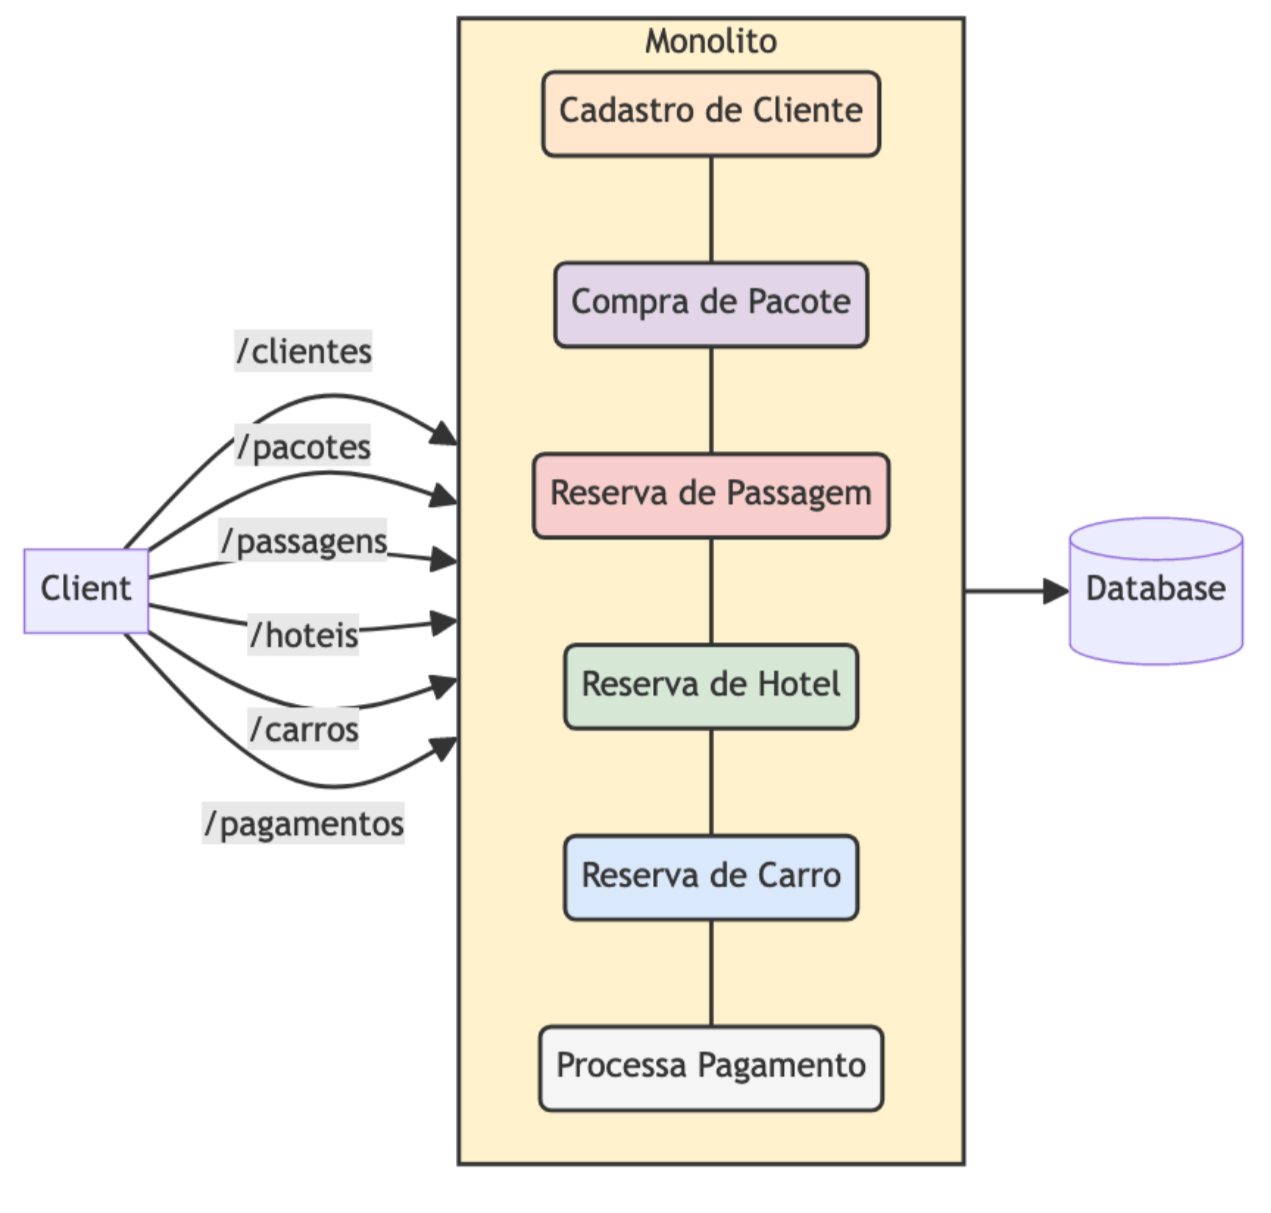
\includegraphics[width=0.8\textwidth]{images/monolito.png}
\caption{Estrutura típica de arquitetura monolítica.}
\label{fig:monolitico}
\end{figure}

Como ilustrado na Figura~\ref{fig:monolitico}, a arquitetura monolítica caracteriza-se pela centralização de todos os módulos e funcionalidades do sistema em uma única aplicação, onde as camadas — como apresentação, lógica de negócio e acesso a dados — encontram-se fortemente acopladas e compartilham o mesmo espaço de execução. O fluxo de requisições percorre camadas internamente acopladas, sem isolamento de processos. Essa centralização, embora simplifique o desenvolvimento inicial, apresenta limitações significativas em cenários de alta demanda e necessidade de escalabilidade.

Segundo Farhan et al.~\cite{farhan2023performance}, sistemas monolíticos apresentaram, em testes empíricos, 40\% maior tempo de resposta sob carga crescente, 68\% mais \textit{downtime} durante atualizações e limite máximo de escalonamento em cinco instâncias, devido ao compartilhamento de recursos e à ausência de isolamento entre processos. Portanto, embora a arquitetura monolítica seja adequada para aplicações de menor porte ou com requisitos estáveis, suas restrições de escalabilidade, resiliência e flexibilidade tornam-se evidentes em ambientes dinâmicos e de grande escala, justificando a busca por alternativas arquiteturais mais modernas.

Portanto, embora a arquitetura monolítica seja adequada para aplicações de menor porte ou com requisitos estáveis, suas restrições de escalabilidade, resiliência e flexibilidade tornam-se evidentes em ambientes dinâmicos e de grande escala, justificando a busca por alternativas arquiteturais mais modernas.

O fluxo de requisições percorre camadas internamente acopladas, sem isolamento de processos. Essa centralização explica os resultados empíricos de \cite{farhan2023performance}, onde sistemas monolíticos apresentaram:
O fluxo de requisições em sistemas monolíticos percorre camadas fortemente acopladas, sem qualquer tipo de isolamento entre processos. Essa centralização estrutural contribui para os resultados observados por \cite{farhan2023performance}, que identificaram um aumento de 40\% no tempo de resposta sob carga crescente, além de 68\% mais \textit{downtime} durante atualizações. Outro dado relevante é o limite máximo de escalonamento, que se restringe a cinco instâncias antes que ocorra degradação crítica do desempenho, evidenciando a dificuldade de adaptação a cenários de alta demanda.

Apesar dessas limitações, a arquitetura monolítica ainda mantém relevância em contextos específicos, como aplicações com tráfego previsível, equipes de desenvolvimento co-localizadas ou situações em que a simplicidade operacional é mais importante do que requisitos de elasticidade \cite{shekhar2023microservices}. No entanto, para sistemas empresariais modernos que exigem entrega contínua, resiliência e escalabilidade dinâmica, a viabilidade do modelo monolítico torna-se progressivamente reduzida, justificando a busca por alternativas arquiteturais mais flexíveis.

\subsection{Event-Driven Architecture}
A \textit{Event-Driven Architecture} é especialmente indicada para sistemas que exigem alta escalabilidade e resposta em tempo real. Nesse padrão, os componentes do sistema comunicam-se por meio de eventos, que são processados de forma assíncrona. Essa abordagem é bastante utilizada em sistemas de \textit{e-commerce}, plataformas de \textit{streaming} e aplicações que demandam processamento distribuído, pois permite maior desacoplamento entre os módulos e facilita a escalabilidade horizontal \cite{jamshidi2016systematic}. 

\subsection{Serverless}
A arquitetura \textit{serverless} tem se destacado com o avanço das plataformas de computação em nuvem, oferecendo uma abordagem inovadora para o desenvolvimento e a execução de aplicações. Nesse modelo, os desenvolvedores podem se concentrar exclusivamente na lógica de negócio, delegando a gestão da infraestrutura ao provedor de nuvem. Essa abstração permite maior agilidade no desenvolvimento e escalabilidade automática, embora apresente desafios relacionados à portabilidade e ao controle sobre o ambiente de execução \cite{shekhar2023microservices}.

\begin{figure}[H]
\centering
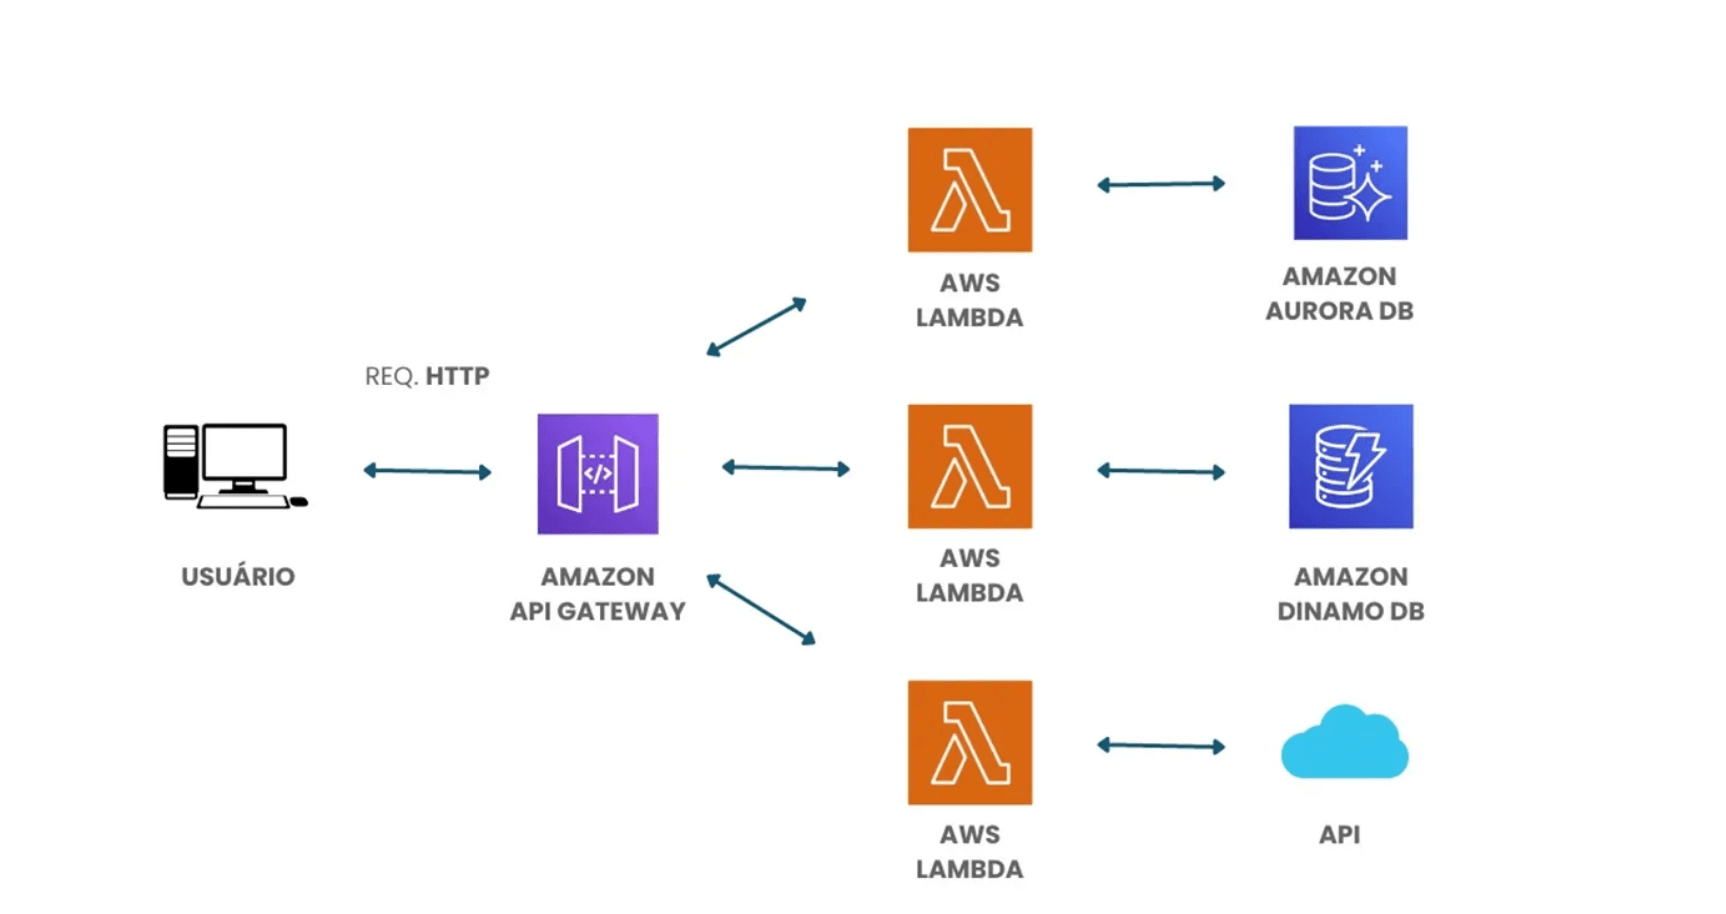
\includegraphics[width=0.9\textwidth]{images/serverless.png}
\caption{Arquitetura Serverless típica, mostrando os componentes principais: API Gateway, Funções como Serviço (FaaS), e serviços gerenciados. Fonte: Adaptado de \cite{shekhar2023microservices}.}
\label{fig:serverless}
\end{figure}

A Figura \ref{fig:serverless} ilustra um exemplo de arquitetura serverless, destacando seus componentes principais. O \textit{API Gateway} atua como o ponto de entrada único para todas as requisições, roteando o tráfego para as funções de backend. As \textit{Funções como Serviço (FaaS)}, como AWS Lambda ou Azure Functions, permitem a execução de código sob demanda, sem a necessidade de provisionar ou gerenciar servidores. Além disso, a arquitetura serverless utiliza \textit{Serviços Gerenciados}, como bancos de dados e filas de mensagens, que são providos e mantidos pelo provedor de nuvem, simplificando ainda mais a operação e a manutenção da aplicação.

A adoção do padrão serverless elimina a necessidade de gerenciamento de servidores, permitindo que os desenvolvedores foquem exclusivamente na implementação da lógica de negócios \cite{shekhar2023microservices}. A escolha do padrão arquitetural mais adequado depende de fatores como requisitos do sistema, contexto de negócio, equipe envolvida e recursos disponíveis. Compreender as vantagens e limitações de cada abordagem é essencial para alinhar a arquitetura às necessidades presentes e futuras do projeto \cite{jamshidi2016systematic, nizami2020comparison}.

\subsection{Microsserviços}
Como abordado anteriormente, a arquitetura de microsserviços decompõe sistemas em serviços autônomos. Sua implementação prática demanda atenção a três dimensões críticas: comunicação, observabilidade e orquestração. \cite{jamshidi2016systematic, nizami2020comparison}. 

Entre os principais benefícios dos microsserviços está a escalabilidade granular, que permite dimensionar apenas os serviços que realmente demandam mais recursos, otimizando custos e desempenho \cite{shekhar2023microservices}. Além disso, a independência entre equipes é favorecida, pois times distintos podem desenvolver, testar e implantar serviços de forma autônoma, acelerando o ciclo de entrega e facilitando a adoção de práticas \textit{DevOps} \cite{nizami2020comparison, farhan2023performance}.

Outro ponto relevante é a resiliência: falhas em um serviço tendem a ser isoladas, reduzindo o impacto sobre o sistema como um todo \cite{farhan2023performance}. Isso é especialmente importante em ambientes de missão crítica, onde a disponibilidade contínua é fundamental. Para garantir essa resiliência, padrões como o \textit{Circuit Breaker} são frequentemente empregados.

Outro ponto relevante é a resiliência: falhas em um serviço tendem a ser isoladas, reduzindo o impacto sobre o sistema como um todo \cite{farhan2023performance}. Isso é especialmente importante em ambientes de missão crítica, onde a disponibilidade contínua é fundamental. Para garantir essa resiliência, padrões como o \textit{Circuit Breaker} são frequentemente empregados.

\begin{figure}[H]
\centering
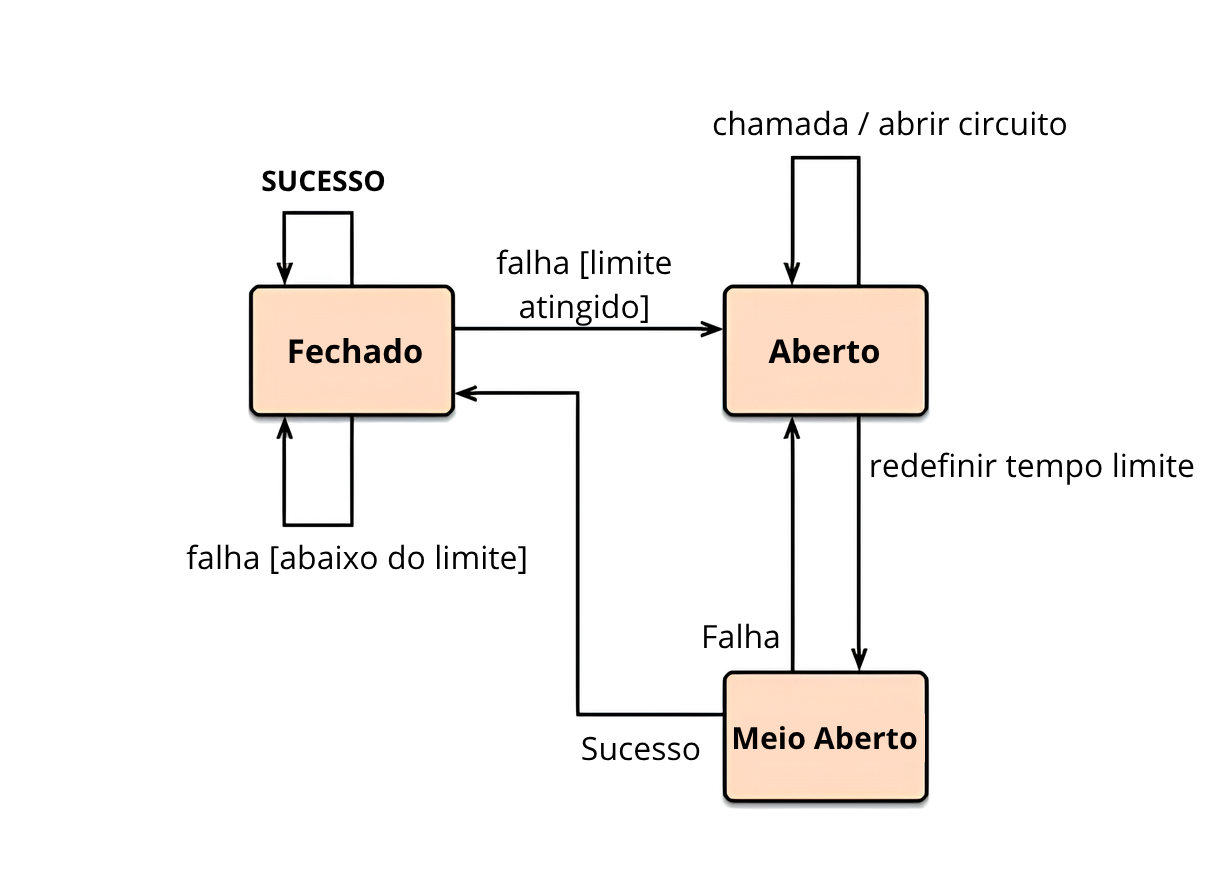
\includegraphics[width=0.7\textwidth]{./images/circuit_breaker.png}
\caption{Funcionamento do padrão Circuit Breaker em sistemas distribuídos.}
\label{fig:circuit-breaker}
\end{figure}

O \textit{Circuit Breaker} é um padrão arquitetural amplamente utilizado em sistemas distribuídos para aumentar a resiliência e evitar falhas em cascata \cite{Nair2019CircuitBreaker, Fowler2012CircuitBreaker}. Ele atua como um "interruptor" que monitora as chamadas a um serviço externo. Seu funcionamento é dividido em três estados principais: fechado, aberto e meio-aberto.

No estado \textbf{fechado}, todas as requisições são encaminhadas normalmente ao serviço. Se o número de falhas ultrapassar um limite configurado, o circuito entra no estado \textbf{aberto}, bloqueando novas tentativas e retornando imediatamente uma resposta de erro ou acionando um mecanismo de \textit{fallback} — uma solução alternativa, como dados em cache ou uma resposta padrão, para manter a aplicação funcionando de forma degradada. Após um tempo de espera, o circuito passa para o estado \textbf{meio-aberto}, permitindo algumas requisições de teste. Se essas requisições forem bem-sucedidas, o circuito retorna ao estado fechado; caso contrário, volta ao estado aberto, protegendo o sistema de sobrecarga e falhas sucessivas \cite{Nair2019CircuitBreaker, Fowler2012CircuitBreaker}.

Esse padrão é fundamental para garantir a robustez de sistemas baseados em microsserviços, pois impede que falhas em um serviço se propaguem e comprometam toda a aplicação. Estudos recentes destacam a importância do \textit{Circuit Breaker} em arquiteturas resilientes, especialmente em ambientes de alta disponibilidade e missão crítica \cite{Nair2019CircuitBreaker}. 

No entanto, a adoção de microsserviços também traz desafios consideráveis. A complexidade operacional aumenta, exigindo ferramentas avançadas para orquestração (como \textit{Kubernetes}), monitoramento e observabilidade \cite{jamshidi2016systematic, shekhar2023microservices}. Cada serviço pode demandar sua própria infraestrutura, banco de dados e mecanismos de autenticação, o que eleva a sobrecarga de gerenciamento \cite{nizami2020comparison}.

A observabilidade torna-se um aspecto central, pois a identificação e resolução de falhas em sistemas distribuídos requerem coleta e análise de métricas, \textit{logs} e \textit{traces} distribuídos \cite{observability2023, sha2023automating}. Ferramentas como \textit{Prometheus} e \textit{Jaeger} são amplamente utilizadas para monitorar o desempenho e rastrear requisições entre serviços, facilitando o diagnóstico de problemas e a manutenção da qualidade do sistema \cite{ahmed2022observability}. 

Além disso, a escolha dos protocolos de comunicação entre microsserviços (\textit{\gls{REST}}, \textit{\gls{gRPC}}, \textit{\gls{GraphQL}}) impacta diretamente o desempenho, a flexibilidade e a observabilidade do sistema \cite{niswar2023performance}. Estudos recentes destacam que decisões arquiteturais bem fundamentadas são essenciais para garantir a eficiência e a robustez de sistemas baseados em microsserviços \cite{niswar2023performance, sha2023automating}. 

A arquitetura de microsserviços representa uma evolução paradigmática no desenvolvimento de software, decompondo sistemas complexos em serviços autônomos especializados. Conforme \cite{jamshidi2016systematic}, esta abordagem oferece:

\begin{itemize}
    \item \textbf{Autonomia tecnológica}: Cada serviço pode utilizar linguagens e tecnologias distintas (Java, Python, Node.js)
    \item \textbf{Resiliência aprimorada}: Isolamento de falhas através de padrões como \textit{Circuit Breaker}
    \item \textbf{Entrega contínua}: \textit{Deploys} independentes permitindo múltiplas implantações diárias
\end{itemize}

\subsubsection{Mecanismos de Comunicação}
A comunicação entre serviços ocorre principalmente através de:

\begin{table}[h]
\centering
\caption{Comparação de protocolos de comunicação}
\begin{tabular}{|l|c|c|c|}
\hline
\textbf{Protocolo} & \textbf{Latência} & \textbf{Complexidade} & \textbf{Casos de Uso} \\
\hline
REST/HTTP & Alta & Baixa & Sistemas com baixa frequência \\
gRPC & Baixa & Média & Microserviços acoplados \\
Eventos (Kafka) & Assíncrona & Alta & Sistemas escaláveis \\
\hline
\end{tabular}
\label{tab:protocolos}
\end{table}

Conforme demonstrado na Tabela \ref{tab:protocolos}, a escolha do protocolo impacta diretamente o desempenho do sistema \cite{niswar2023performance}.

\subsubsection{Padrões Arquiteturais Essenciais}
\begin{figure}[H]
\centering
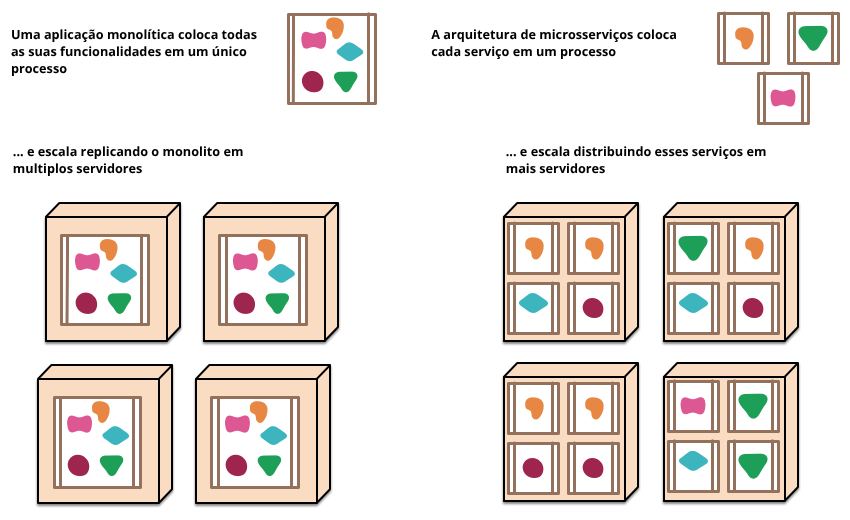
\includegraphics[width=0.85\textwidth]{images/microservice.png}
\caption{Padrões fundamentais em arquitetura de microsserviços}
\label{fig:micro_patterns}
\end{figure}

A Figura \ref{fig:micro_patterns} ilustra as diferenças fundamentais entre a arquitetura monolítica e a arquitetura de microsserviços. À esquerda, observa-se que uma aplicação monolítica agrupa todas as funcionalidades em um único processo. Para escalar esse modelo, é necessário replicar toda a aplicação em múltiplos servidores, o que pode gerar desperdício de recursos e limitações de flexibilidade.

À direita, a arquitetura de microsserviços distribui cada funcionalidade em processos independentes, permitindo que cada serviço seja desenvolvido, implantado e escalado separadamente. Isso proporciona maior eficiência no uso de recursos, facilita a manutenção e possibilita o crescimento gradual do sistema conforme a demanda por funcionalidades específicas.

Essa abordagem modular e distribuída é um dos pilares das arquiteturas modernas voltadas à escalabilidade, resiliência e agilidade no desenvolvimento.

\subsubsection{Desafios Operacionais e Soluções}
A implementação prática enfrenta obstáculos significativos:

\begin{itemize}
    \item \textbf{Observabilidade}: Requer integração de métricas, \textit{logs} e \textit{traces} com ferramentas como:
    \begin{itemize}
        \item \textit{Prometheus} para monitoramento
        \item \textit{Jaeger} para rastreamento distribuído
        \item \textit{EFK Stack} (Elasticsearch, Fluentd, Kibana) para análise
    \end{itemize}
    
    \item \textbf{Orquestração}: Plataformas como \textit{Kubernetes} gerenciam:
    \begin{itemize}
        \item Escalonamento automático
        \item Balanceamento de carga
        \item Recuperação de falhas
    \end{itemize}
\end{itemize}

\subsubsection{Melhores Práticas de Implementação}
Experiências de empresas líderes revelam estratégias eficazes:

\begin{itemize}
    \item \textbf{Amazon}: Utiliza a prática do "time da pizza de dois" — equipes pequenas e independentes, responsáveis por serviços autônomos do início ao fim.
    
    \item \textbf{Netflix}: Introduziu a cultura do \textit{Chaos Engineering}, simulando falhas em produção para garantir a resiliência dos serviços.

    \item \textbf{Spotify}: Estruturou suas equipes em \textit{squads} responsáveis por domínios funcionais, promovendo independência e entrega contínua.

    \item \textbf{Uber}: Implementou uma hierarquia de serviços baseada em criticidade, diferenciando serviços centrais de auxiliares para otimizar a operação.
\end{itemize}

\subsubsection{Casos de Estudo Relevantes}
Resultados empíricos demonstram impactos mensuráveis:

\begin{table}[h]
\centering
\caption{Impacto da migração para microsserviços}
\begin{tabular}{|l|c|c|}
\hline
\textbf{Métrica} & \textbf{Antes} & \textbf{Depois} \\
\hline
Tempo de entrega & 30 dias & 2 dias \\
Disponibilidade & 92\% & 99.95\% \\
Custo de infraestrutura & \$100k/mês & \$65k/mês \\
\hline
\end{tabular}
\label{tab:impacto}
\end{table}

Conforme dados na Tabela \ref{tab:impacto}, organizações reportam melhorias significativas após transição bem-sucedida \cite{farhan2023performance, shekhar2023microservices}.

\subsubsection{Recomendações Estratégicas}
A adoção deve considerar:

\begin{itemize}
    \item \textbf{Pré-requisitos}: Maturidade em DevOps e cultura de automação
    \item \textbf{Critérios}: Complexidade sistêmica > 50k LOC > 15 desenvolvedores
    \item \textbf{Alternativas}: Arquiteturas híbridas para transição gradual
    \item \textbf{Anti-padrões}: Decomposição excessiva ("nanoserviços")
\end{itemize}

Em síntese, microsserviços oferecem vantagens transformacionais para sistemas complexos, mas exigem investimento proporcional em automação e governança \cite{nizami2020comparison, observability2023}.

\subsection{Protocolos de Comunicação para Microsserviços}
A seleção de protocolos de comunicação é um fator crítico em arquiteturas de microsserviços, influenciando diretamente o desempenho, acoplamento e capacidade de evolução do sistema. Dois padrões predominantes neste contexto são \gls{REST} e \gls{gRPC}, cada um com características técnicas distintas que os tornam adequados a cenários específicos \cite{niswar2023performance}.

\subsubsection{\gls{REST} (Representational State Transfer)}
O \gls{REST}, formalizado por Fielding \cite{fielding2000rest} em sua tese seminal, é um estilo arquitetural baseado em princípios de recursos identificáveis por \gls{URI} e operações padronizadas via verbos \gls{HTTP} (GET, POST, PUT, DELETE). Sua adoção generalizada deve-se a:

\begin{itemize}
\item \textbf{Simplicidade}: Uso de formatos legíveis como \gls{JSON}, facilitando depuração e integração entre sistemas heterogêneos. A serialização textual consome 30-50\% mais banda que protocolos binários \cite{niswar2023performance}.
\item \textbf{Estateless}: Cada requisição contém contexto completo, eliminando estado no servidor e favorecendo escalabilidade horizontal \cite{fielding2000rest}.
\item \textbf{Uniform Interface}: Princípios como identificação única de recursos via URI e \gls{HATEOAS} garantem consistência e desacoplamento \cite{maso2024comparativo}.
\item \textbf{Compatibilidade}: Suporte nativo em navegadores e adoção massiva em APIs públicas \cite{maso2024comparativo}.
\end{itemize}

\textbf{Limitações em cenários complexos}:
\begin{itemize}
\item \textbf{Overhead de comunicação}: Serialização textual aumenta latência e consumo de \gls{CPU}, especialmente em payloads grandes \cite{niswar2023performance}.
\item \textbf{Modelo síncrono}: Suporta apenas comunicação unária (request/response), inviabilizando fluxos assíncronos \cite{niswar2023performance}.
\item \textbf{Falta de contratos rígidos}: Validação de esquemas depende de implementações adicionais \cite{maso2024comparativo}.
\end{itemize}

\textbf{Operações Básicas e Códigos HTTP}:
A Tabela \ref{tab:rest_operations} sintetiza o mapeamento CRUD em REST, conforme padrões industriais \cite{fielding2000rest}:

\begin{table}[h]
\centering
\caption{Operações REST e códigos HTTP}
\label{tab:rest_operations}
\begin{tabular}{|l|c|c|}
\hline
\textbf{Método HTTP} & \textbf{Ação} & \textbf{Código Sucesso} \\ \hline
GET & Ler recurso & 200 (OK) \\ \hline
POST & Criar recurso & 201 (Created) \\ \hline
PUT/PATCH & Atualizar recurso & 200 (OK) ou 204 (No Content) \\ \hline
DELETE & Excluir recurso & 204 (No Content) \\ \hline
\end{tabular}
\fonte{Adaptado de \cite{niswar2023performance} e \cite{fielding2000rest}.}
\end{table}

% \begin{figure}[h]
% \centering
% \includegraphics[width=0.75\textwidth]{images/rest-protocol.png}
% \caption{Fluxo de comunicação REST típico com operações CRUD sobre recursos. Fonte: Adaptado de \cite{aws:1}.}
% \label{fig:rest_flow}
% \end{figure}

\subsubsection{\gls{gRPC} (gRPC Remote Procedure Calls)}
Desenvolvido pelo Google e inicialmente lançado em 2015 \cite{googleblog:5}, o \gls{gRPC} é um \textit{framework} aberto de alta performance para chamadas de procedimento remoto (RPC) que utiliza \gls{HTTP/2} e \textit{Protocol Buffers} para comunicação binária eficiente. Conforme demonstrado por \cite{niswar2023performance}, sua adoção em arquiteturas de microsserviços deve-se aos seguintes diferenciais:

\begin{itemize}
\item \textbf{Desempenho superior}: A serialização binária via \textit{Protocol Buffers} reduz o tamanho dos \textit{payloads} em até 80\% e a latência em 60\% comparado a APIs REST tradicionais, conforme mensurações em ambientes controlados \cite{niswar2023performance}.
\item \textbf{Streaming bidirecional}: Suporte nativo a fluxos contínuos de dados (cliente-servidor, servidor-cliente e bidirecional), habilitando comunicação assíncrona para aplicações em tempo real \cite{grpc:1}.
\item \textbf{Contratos fortemente tipados}: Definição explícita de serviços e estruturas de mensagens em arquivos \texttt{.proto}, garantindo compatibilidade e evolução controlada de APIs \cite{maso2024comparativo}.
\item \textbf{Geração de código automática}: Compilação de \textit{stubs} clientes e servidores em 11 linguagens de programação a partir de arquivos \texttt{.proto}, promovendo consistência e redução de erros \cite{grpc:1}.
\end{itemize}

\textbf{Aspectos críticos em sua adoção}:
\begin{itemize}
\item \textbf{Acoplamento forte}: Alterações nos contratos \texttt{.proto} exigem atualização sincronizada de clientes e servidores, aumentando a complexidade de evolução em sistemas distribuídos \cite{ibm:7}.
\item \textbf{Suporte limitado em navegadores}: A ausência de implementação nativa do HTTP/2 em navegadores requer o uso do proxy \textit{gRPC-Web} para comunicações cliente-web \cite{wallarm:4}.
\item \textbf{Curva de aprendizagem}: Complexidade na definição de contratos e manipulação de fluxos de \textit{streaming}, especialmente para desenvolvedores familiarizados com paradigmas REST \cite{marutitech:9}.
\end{itemize}

\textbf{Modelos de Comunicação}:
A Figura \ref{fig:grpc_streaming} ilustra os quatro padrões suportados:

\begin{figure}[H]
\centering
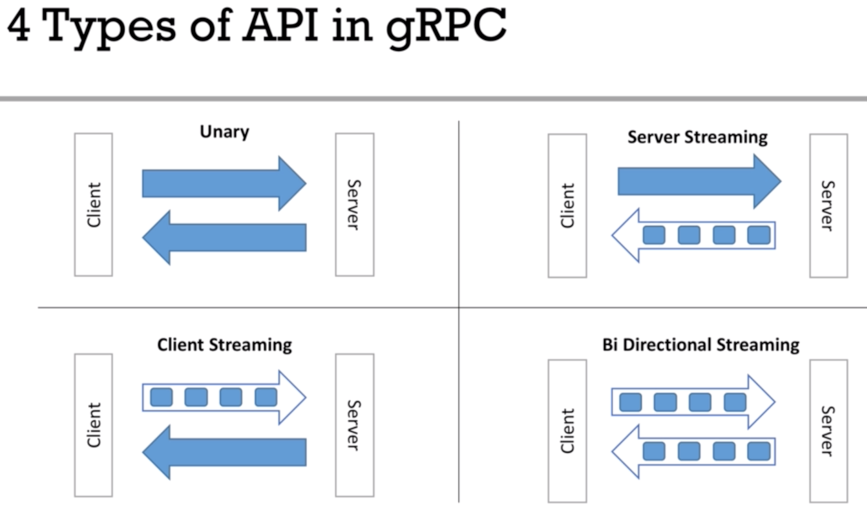
\includegraphics[width=0.9\textwidth]{images/grpc.png}
\caption{Padrões de streaming no gRPC: (A) Unário, (B) Servidor, (C) Cliente, (D) Bidirecional.}
\label{fig:grpc_streaming}
\end{figure}

\textbf{Vantagens Técnicas Comprovadas}:
Estudos empíricos demonstram ganhos operacionais mensuráveis \cite{niswar2023performance}:
\begin{itemize}
\item Redução de 35-45\% no consumo de CPU durante serialização
\item Até 7x maior throughput em comunicações inter-serviços
\end{itemize}

% \ref{cap:Introducao}).
% \ref{cap:Introducao}).
% % ----------------------------------------------------------
% \section{CONCEITOS EXPLORADOS NO TRABALHO}\label{sec:conceitos}
% % ----------------------------------------------------------

% Para cada conceito explorado no trabalho, você deve criar nova uma seção como esta, por exemplo: “2.1 INTERNET DAS COISAS”.

% % ----------------------------------------------------------
% \section{TECNOLOGIAS UTILIZADAS NO DESENVOLVIMENTO}\label{sec:tecnologias}
% % ----------------------------------------------------------

% Para cada tecnologia utilizada no desenvolvimento, você deve criar uma nova seção como esta, por exemplo: “2.2 PLATAFORMA ARDUINO”.

% ----------------------------------------------------------
% \section{Exemplo citação longa em Látex} \label{}
% ----------------------------------------------------------


% \begin{citacao}
% 	Após a ilustração, na parte inferior, indicar a fonte consultada (elemento obrigatório, mesmo que seja produção do próprio autor), legenda, notas e outras informações necessárias à sua compreensão (se houver). A ilustração deve ser citada no texto e inserida o mais próximo possível do texto a que se refere. \cite[p. 11]{gil2008metodos}.
% \end{citacao}

% % ----------------------------------------------------------
% \section{Exemplo Equações e fórmulas em Látex}
% % ----------------------------------------------------------

% As equações e fórmulas devem ser destacadas no texto para facilitar a leitura. Para numerá-las, usar algarismos arábicos entre parênteses e alinhados à direita. Pode-se adotar uma entrelinha maior do que a usada no texto.

% Exemplos, \ref{eq:Eq_1} e \ref{eq:Eq_2}.

% \begin{equation}\label{eq:Eq_1}
% C = 2 \pi r
% \end{equation}

% \begin{equation}\label{eq:Eq_2}
% \gls{A} = \gls{pi} \gls{r}^2
% \end{equation}


% % ----------------------------------------------------------
% \section{Exemplo Código-Fonte}
% % ----------------------------------------------------------

% Os trechos de código devem ser exibidos em formatação de código com linhas enumeradas sequenciais a esquerda para falicitar os comentários. Abaixo segue exemplos carregando o código através de um arquivo e digitando diretamente no texto.

% \lstinputlisting[
%     language=C, % Defina a linguagem do código
%     numbers=left, % Exibir números de linha à esquerda
%     %linerange={23-66}, % Defina os intervalos de linhas
%     firstnumber={1}, % Números iniciais correspondentes aos intervalos
%     stepnumber=1, % Incremento do número de linha
%     caption={Exemplo carregando arquivo...},
%     label=src:sample_c
% ]{sources/sample.c}

% \begin{lstlisting}[language=json, caption={Exemplo de Dados JSON}, label={src:json}]
%     {
%         "name": "John Doe",
%         "age": 30,
%         "address": {
%             "street": "1234 Main St",
%             "city": "Anytown",
%             "state": "CA",
%             "zip": "12345"
%         },
%         "phoneNumbers": [
%             {"type": "home", "number": "555-1234"},
%             {"type": "work", "number": "555-5678"}
%         ]
%     }
%     \end{lstlisting}


% \begin{lstlisting}[language=C, caption={Exemplo digitado no texto}, label={src:codigo_2}]
% 	#include <stdio.h>
	
% 	void main(){
% 		printf("Olá Mundo!");
% 	}
% 	\end{lstlisting}

% Exemplos, \ref{src:sample_c}, \ref{src:json} e \ref{src:codigo_2}.


% ----------------------------------------------------------
\chapter{DESENVOLVIMENTO} \label{cap:desenvolvimento}
% ----------------------------------------------------------

% A estrutura de seções deste capítulo varia em função das características de cada trabalho, e deve ser definida junto com o orientador no decorrer da disciplina. A seguir é apresentada uma estrutura de seções tradicionalmente utilizada em TCCs que envolvem o desenvolvimento de um software. 


% ----------------------------------------------------------
% \section{VISÃO GERAL DO PROJETO}\label{sec:visao}
% % ----------------------------------------------------------

% Em alguns casos, pode ser interessante fornecer ao leitor uma visão geral do projeto, especialmente quando a solução é complexa e/ou envolve diversos componentes. Você também pode utilizar esta seção para falar um pouco sobre o modelo de processo de software adotado (cascata, espiral, incremental, …) e o planejamento das atividades realizadas.

% \begin{figure}[htb]
% 	\begin{center}
% 		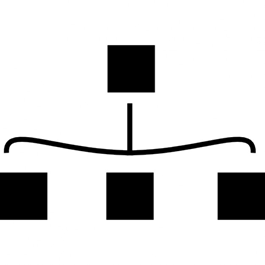
\includegraphics{images/figura1.png}
% 	\end{center}
% 	\caption{\label{fig:Fig_1}Visão geral do projeto}
% 	\fonte{Elaborado pelo autor deste trabalho (2018).}
% \end{figure}

% A Figura \ref{fig:Fig_1} representa ...

% ----------------------------------------------------------
% \section{LEVANTAMENTO DE REQUISITOS} \label{sec:requisitos}
% ----------------------------------------------------------

% Você pode iniciar esta seção explicando como e quando foram levantados os requisitos do sistema. Entrevistas com os proprietários da empresa? Documentação do software legado? Questionários aplicados aos usuários?

% Em seguida você deve apresentar a especificação dos Requisitos Funcionais, Requisitos Não Funcionais e Regras de Negócio do sistema, conforme os ensinamentos da disciplina de Engenharia de Software, por exemplo:

% A partir das entrevistas com os proprietários da empresa, foram identificados os seguintes requisitos funcionais para o sistema a ser desenvolvido:

% \textbf{RF01} – O sistema deverá permitir ao usuário manter produtos;

% \textbf{RF02} – O sistema deverá permitir ao usuário administrador manter categorias de produtos;

% \textbf{RF03} – ...

% Os seguintes requisitos não funcionais:

% \textbf{RNF01} – Todas as funcionalidades serão executadas online, ou seja, através de acesso a um servidor web;

% \textbf{RNF02} – Os dados serão armazenados em banco de dados MySQL;

% \textbf{RNF03} – As linguagens para implementação são: HTML5, CSS, Javascript, jQuery e PHP;

% \textbf{RNF04} – A interface gráfica com o usuário deve ser compatível com telas de computadores desktop, tablets e smartphones, e empregar o conceito de Web Design Responsivo através do framework Bootstrap.

% \textbf{RNF05} – ...

% E as seguintes regras de negócio:

% \textbf{RN01} – A venda a prazo só poderá ser feita para clientes adimplentes;

% \textbf{RN02} – ...

% ----------------------------------------------------------
% \section{MODELAGEM}
% ----------------------------------------------------------

% A estrutura de subseções a seguir varia em função das características de cada trabalho, e deve ser definida junto com o orientador no decorrer da disciplina. Os digramas comumente utilizados em TCCs que envolvem o desenvolvimento de um software são: diagrama de casos de uso, modelo de dados, diagrama de classes, diagrama de atividades, diagrama de sequência e diagrama de componentes. Normalmente, dois ou três desses diagramas são suficientes para fornecer as visões necessárias do projeto.

% ----------------------------------------------------------
% \subsection{Casos de uso} 
% ----------------------------------------------------------

% Caso o seu projeto utilize o diagrama de casos de uso (Figura \ref{fig:Fig_2}), é importante que ele esteja coerente com os requisitos funcionais (RFs) apresentados no levantamento de requisitos (Seção \ref{sec:requisitos}). Também é importante utilizar corretamente as notações UML, tais como “include”, “extend” e “generalization”. Não se esqueça de explicar o diagrama após a ilustração, conforme o exemplo a seguir.

% \begin{figure}[htb]
% 	\begin{center}
% 		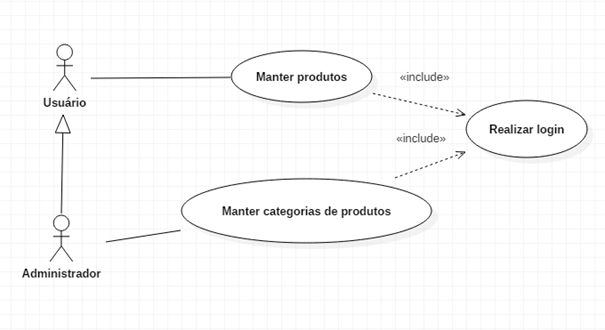
\includegraphics{images/figura2.png}
% 	\end{center}
% 	\caption{\label{fig:Fig_2}Diagrama de casos de uso}
% 	\fonte{Elaborado pelo autor deste trabalho com o uso da ferramenta StarUML (2018).}
% \end{figure}

% O usuário do tipo administrador herda as funcionalidades do usuário comum... 

% Para executar as funcionalidades, os usuários devem realizar o login...

% A documentação dos casos de uso encontra-se no Apêndice A deste trabalho.

% % ----------------------------------------------------------
% \subsection{Modelos de dados}
% % ----------------------------------------------------------

% O modelo de dados é um diagrama que descreve o esquema do banco de dados. Caso o seu projeto utilize este tipo de diagrama, não se esqueça de explicá-lo após a ilustração, conforme o exemplo a seguir.

% \begin{figure}[htb]
%     \begin{center}
% 	    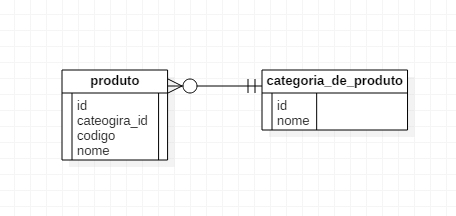
\includegraphics{images/figura3.png}
% 	\end{center}
% 	\caption{\label{fig:Fig_3}Modelo de banco de dados}
% 	\fonte{Elaborado pelo autor deste trabalho com o uso da ferramenta StarUML (2018).}
% \end{figure}

% O esquema de banco de dados é composto de duas tabelas...Os campos do tipo “id” são utilizados para...

% O código SQL de construção do esquema de banco de dados encontra-se no Apêndice B deste trabalho.

% ----------------------------------------------------------
\subsection{IMPLEMENTAÇÃO}
% ----------------------------------------------------------

Nesta seção você pode falar um pouco sobre o código desenvolvido. Não é necessário explicar ou apresentar todo o código fonte da aplicação. Você pode focar nas principais classes ou funções. É importante explicar quais foram as ferramentas utilizadas e o porquê da escolha de cada uma delas.

Você deve colocar o código na pasta sources e carrega-lo ao apêndice, usando aqui apenas uma referência ou trechos de código.

O código presente no Apêndice \ref{apendice:b} representa ....
% ----------------------------------------------------------
\chapter{TESTE OU AVALIAÇÃO} \label{cap:teste}
% ----------------------------------------------------------

Testes e avaliações tem o poder de enriquecer o trabalho acadêmico, fornecendo dados que permitirão ao leitor avaliar a qualidade da solução desenvolvida. Este capítulo pode apresentar, por exemplo, um teste de usabilidade com três seções: 4.1 PLANEJAMENTO, 4.2 EXECUÇÃO e 4.3 RESULTADOS.
Como outro exemplo, este capítulo pode apresentar um estudo de caso ou simulação com o uso da solução desenvolvida. Neste caso, uma possível estrutura de seções seria: 4.1 AMBIENTE DE ESTUDO, 4.2 IMPLANTAÇÃO, 4.3 RESULTADOS.
Para apresentação de dados ou estatísticas, utilize tabelas, lembrando que, diferente das ilustrações, as legendas das tabelas aparecem na parte superior.

% \begin{table}[htb]
% 	\ABNTEXfontereduzida
% 	\caption{\label{tab:Tab_1}Exemplo de tabela em Látex.}
% 	\begin{tabular}{@{}p{3.0cm}p{1.5cm}p{2cm}p{2.5cm}p{2.5cm}p{2.5cm}@{}}
% 		\toprule
% 		\textbf{Média concentração urbana} & \multicolumn{2}{l}{\textbf{População}} & \textbf{Produto Interno Bruto – PIB (bilhões R\$)} & \textbf{Número de empresas} & \textbf{Número de unidades locais} \\ \midrule
% 		\textbf{Nome}                      & \textbf{Total}   & \textbf{No Brasil}  &                                                   &                             & \\
% 		Ji-Paraná (RO)                     & 116 610          & 116 610             & 1,686                                             & 2 734                       & 3 082 \\
% 		Parintins (AM)                     & 102 033          & 102 033             & 0,675                                             & 634                         & 683 \\
% 		Boa Vista (RR)                     & 298 215          & 298 215             & 4,823                                             & 4 852                       & 5 187 \\
% 		Bragança (PA)                      & 113 227          & 113 227             & 0,452                                             & 654                         & 686 \\ \bottomrule
% 	\end{tabular}
% 	\fonte{Elaborado pelo autor deste trabalho (2018).}
% \end{table}
% ----------------------------------------------------------
\chapter{CONSIDERAÇÕES FINAIS} \label{cap:consideracoes}
% ----------------------------------------------------------

Você deve iniciar as considerações “olhando” para os objetivos apresentados na Seção \ref{sec:objetivos}. Inicie falando sobre como os objetivos foram alcançados.
Em seguida fale sobre as suas experiências e descobertas ao realizar o trabalho, por exemplo, as vantagens e desvantagens das tecnologias utilizadas e as dificuldades encontradas no desenvolvimento da solução.
Encerre as considerações com narrativas mais gerais, expondo sua visão do trabalho como um todo.

% ----------------------------------------------------------
\section{CONTRIBUIÇÕES} 
% ----------------------------------------------------------

Quais foram as constituições do seu trabalho? É importante destacar que não são contribuições para você, mas sim para quem irá utilizar o trabalho como referência! Por exemplo, você pode citar como contribuições os estudos, especificações, modelos e outros recursos disponíveis no trabalho e que podem ser utilizados por terceiros como base para o desenvolvimento de novos trabalhos ou pesquisas.

% ----------------------------------------------------------
\section{TRABALHOS FUTUROS} 
% ----------------------------------------------------------

Listar o que pode ser melhorado ou adicionado na solução desenvolvida.

% \gls{Palavra}

% \gls{OutraPalavra}

% ----------------------------------------------------------
% ELEMENTOS PÓS-TEXTUAIS
% ----------------------------------------------------------
\postextual
% ----------------------------------------------------------

% ----------------------------------------------------------
% Referências bibliográficas
% ----------------------------------------------------------
\begingroup
    \printbibliography[title=REFERÊNCIAS]
\endgroup

% ----------------------------------------------------------
% Glossário
% ----------------------------------------------------------
\imprimirglossario

% ----------------------------------------------------------
% Apêndices
% ----------------------------------------------------------

% ---
% Inicia os apêndices
% ---
\begin{apendicesenv}
	%\partapendices* 
	% ----------------------------------------------------------
\chapter{Descrição 1}\label{apendice:a}
% ----------------------------------------------------------

Textos elaborados pelo autor, a fim de completar a sua argumentação. Deve ser precedido da palavra APÊNDICE, identificada por letras maiúsculas consecutivas, travessão e pelo respectivo título. Utilizam-se letras maiúsculas dobradas quando esgotadas as letras do alfabeto. 

	% ----------------------------------------------------------
\chapter{Código Fonte}\label{apendice:b}
% ----------------------------------------------------------

%Carregando código fonte da pasta sources no apêndice 

\lstinputlisting[
    language=C, % Defina a linguagem do código
    numbers=left, % Exibir números de linha à esquerda
    firstnumber={1}, % Números iniciais correspondentes aos intervalos
    stepnumber=1, % Incremento do número de linha
    caption={Exemplo carregando arquivo...},
    label=src:sample_c
]{sources/sample.c}
\end{apendicesenv}
% ---


% ----------------------------------------------------------
% Anexos
% ----------------------------------------------------------

% ---
% Inicia os anexos
% ---
\begin{anexosenv}
	%\partanexos*
	% ----------------------------------------------------------
\chapter{Declaração de Isenção}\label{anexo:a}
% ----------------------------------------------------------

\begin{center}
    \textbf{DECLARAÇÃO DE ISENÇÃO}
\end{center}

\vspace{1cm}

\imprimirlocal,~\imprimirdata.

\vspace{1cm}

Declaro, para todos os fins de direito, que assumo total responsabilidade pelo aporte ideológico conferido ao presente trabalho, estando ciente do disposto, da Resolução CONSUN 46-2019 e, isentando o Centro Universitário Avantis, o Curso de Sistemas de Informação, a Banca Examinadora e o Orientador de Trabalho de Conclusão de Curso de toda e qualquer responsabilidade acerca do mesmo.\\
\vspace{5cm}
\begin{center}

\assinatura{\MakeTextUppercase{\textbf{\imprimirautor}}}
\end{center}


\end{anexosenv}

%---------------------------------------------------------------------
% INDICE REMISSIVO
%---------------------------------------------------------------------
% \phantompart
% \printindex
%---------------------------------------------------------------------

\end{document}
